%%%% begin for word count from icer website %%%%
%TC:macro \cite [option:text,text]
%TC:macro \citep [option:text,text]
%TC:macro \citet [option:text,text]
%TC:envir table 0 1
%TC:envir table* 0 1
%TC:envir tabular [ignore] word
%TC:envir displaymath 0 word
%TC:envir math 0 word
%TC:envir comment 0 0

%%%% end for word count %%%%

%%
%% This is file `sample-manuscript.tex',
%% generated with the docstrip utility.
%%
%% The original source files were:
%%
%% samples.dtx  (with options: `manuscript')
%% 
%% IMPORTANT NOTICE:
%% 
%% For the copyright see the source file.
%% 
%% Any modified versions of this file must be renamed
%% with new filenames distinct from sample-manuscript.tex.
%% 
%% For distribution of the original source see the terms
%% for copying and modification in the file samples.dtx.
%% 
%% This generated file may be distributed as long as the
%% original source files, as listed above, are part of the
%% same distribution. (The sources need not necessarily be
%% in the same archive or directory.)
%%
%% Commands for TeXCount
%TC:macro \cite [option:text,text]
%TC:macro \citep [option:text,text]
%TC:macro \citet [option:text,text]
%TC:envir table 0 1
%TC:envir table* 0 1
%TC:envir tabular [ignore] word
%TC:envir displaymath 0 word
%TC:envir math 0 word
%TC:envir comment 0 0
%%
%%
%% The first command in your LaTeX source must be the \documentclass command.
%%%% Small single column format, used for CIE, CSUR, DTRAP, JACM, JDIQ, JEA, JERIC, JETC, PACMCGIT, TAAS, TACCESS, TACO, TALG, TALLIP (formerly TALIP), TCPS, TDSCI, TEAC, TECS, TELO, THRI, TIIS, TIOT, TISSEC, TIST, TKDD, TMIS, TOCE, TOCHI, TOCL, TOCS, TOCT, TODAES, TODS, TOIS, TOIT, TOMACS, TOMM (formerly TOMCCAP), TOMPECS, TOMS, TOPC, TOPLAS, TOPS, TOS, TOSEM, TOSN, TQC, TRETS, TSAS, TSC, TSLP, TWEB.
% \documentclass[acmsmall]{acmart}

%%%% Large single column format, used for IMWUT, JOCCH, PACMPL, POMACS, TAP, PACMHCI
% \documentclass[acmlarge,screen]{acmart}

%%%% Large double column format, used for TOG
% \documentclass[acmtog, authorversion]{acmart}

%%%% Generic manuscript mode, required for submission
%%%% and peer review
\documentclass[manuscript, review,screen,sigconf]{acmart}
%% Fonts used in the template cannot be substituted; margin 
%% adjustments are not allowed.
%%
%% \BibTeX command to typeset BibTeX logo in the docs
\AtBeginDocument{%
  \providecommand\BibTeX{{%
    \normalfont B\kern-0.5em{\scshape i\kern-0.25em b}\kern-0.8em\TeX}}}

%% Rights management information.  This information is sent to you
%% when you complete the rights form.  These commands have SAMPLE
%% values in them; it is your responsibility as an author to replace
%% the commands and values with those provided to you when you
%% complete the rights form.
\setcopyright{acmcopyright}
\copyrightyear{2024}
\acmYear{2024}
\acmDOI{XXXXXXX.XXXXXXX}

\acmConference[ICER 2024]{}{August 13--15, 2024}{ Melbourne, Victoria, Australia}
%
%  Uncomment \acmBooktitle if th title of the proceedings is different
%  from ``Proceedings of ...''!
%
\acmBooktitle{} 
\acmPrice{}
\acmISBN{}

%%
%% Submission ID.
%% Use this when submitting an article to a sponsored event. You'll
%% receive a unique submission ID from the organizers
%% of the event, and this ID should be used as the parameter to this command.
%%\acmSubmissionID{123-A56-BU3}

%%
%% The majority of ACM publications use numbered citations and
%% references.  The command \citestyle{authoryear} switches to the
%% "author year" style.
%%
%% If you are preparing content for an event
%% sponsored by ACM SIGGRAPH, you must use the "author year" style of
%% citations and references.
%% Uncommenting
%% the next command will enable that style.
%%\citestyle{acmauthoryear}

%%
%% end of the preamble, start of the body of the document source.
\usepackage{enumitem}
\usepackage{hyperref}
\usepackage{comment}
\usepackage{mdframed}

\usepackage{graphicx}
\usepackage{caption}
\usepackage{subcaption}

\begin{document}

%%
%% The "title" command has an optional parameter,
%% allowing the author to define a "short title" to be used in page headers.
\title[Influence of Personality Traits on Plagiarism Through Collusion in Programming Assignments]{Influence of Personality Traits on Plagiarism Through Collusion in Programming Assignments}

%%
%% The "author" command and its associated commands are used to define
%% the authors and their affiliations.
%% Of note is the shared affiliation of the first two authors and the
%% "authornote" and "authornotemark" commands
%% used to denote shared contribution to the research.
 
%%\author{P D Parthasarathy}\email{p20210042@goa.bits-pilani.ac.in}\orcid{0000-0002-8723-2407}
%%\affiliation{%
%%\institution{BITS Pilani, KK Birla Goa Campus}
%%\city{}\state{Goa}
%%\country{India}
%%\postcode{403726}
%%}
%%\author{Swaroop Joshi}\email{swaroopj@goa.bits-pilani.ac.in}\orcid{0000-0003-4536-2446}
%%\affiliation{%
%%  \institution{BITS Pilani, KK Birla Goa Campus}
%%  \city{}\state{Goa}
%%  \country{India}
%%  \postcode{403726}
%%}
%%\author{Dev Goel}\email{f20190236@goa.bits-pilani.ac.in}\orcid{0009-0006-4775-4776}
%%\affiliation{%
%%  \institution{BITS Pilani, KK Birla Goa Campus}
%%  \city{}\state{Goa}
%%  \country{India}
%%  \postcode{403726}

\author{First author}\email{email@email}\orcid{0000-0000-0000-0000}
\affiliation{%
  \institution{Univerisity Name}
  \city{}\state{State}
  \country{Country}
  \postcode{Code}
}
\author{Second author}\email{email@email}\orcid{0000-0000-0000-0000}
\affiliation{%
  \institution{Univerisity Name}
  \city{}\state{State}
  \country{Country}
  \postcode{Code}
}
\author{Third author}\email{email@email}\orcid{0000-0000-0000-0000}
\affiliation{%
  \institution{Univerisity Name}
  \city{}\state{State}
  \country{Country}
  \postcode{Code}
}

%% By default, the full list of authors will be used in the page
%% headers. Often, this list is too long, and will overlap
%% other information printed in the page headers. This command allows
%% the author to define a more concise list
%% of authors' names for this purpose.
\renewcommand{\shortauthors}{}

%%
%% The abstract is a short summary of the work to be presented in the
%% article.
\begin{abstract}
    Advancements in Generative-AI and large language models have increased concerns about academic dishonesty and plagiarism in take-home assignments within computing education. Extensive research has linked key traits from the Big Five personality model to various forms of anti-social behavior. However, there is a notable gap in research regarding the association between personality traits and plagiarism, particularly in programming assignments within computing education. This study addresses this gap by investigating the relationship between the Big Five personality traits and plagiarism scores in programming assignments among undergraduate students. The study was conducted in an artificial intelligence course with 105 participants (N=105) at a large private university in India. Additionally, the study explores whether educating students about academic integrity and clearly defining plagiarism expectations affect plagiarism rates. Our findings suggest that while educating students about plagiarism has a limited impact on reducing malpractice in programming assignments, the extraversion trait of the Big Five personality exhibits a positive association and the conscientiousness trait exhibits a negative association with plagiarism tendencies.
\end{abstract}

%%
%% The code below is generated by the tool at http://dl.acm.org/ccs.cfm.
%% Please copy and paste the code instead of the example below.
%%
\begin{CCSXML}
<ccs2012>
   <concept>
       <concept_id>10003456.10003457.10003527.10003540</concept_id>
       <concept_desc>Social and professional topics~Student assessment</concept_desc>
       <concept_significance>300</concept_significance>
       </concept>
   <concept>
       <concept_id>10003456.10003462.10003463</concept_id>
       <concept_desc>Social and professional topics~Intellectual property</concept_desc>
       <concept_significance>500</concept_significance>
       </concept>
 </ccs2012>
\end{CCSXML}

\ccsdesc[300]{Social and professional topics~Student assessment}
\ccsdesc[500]{Social and professional topics~Intellectual property}

\ccsdesc[500]{Social and professional topics~Computing education}

%%
%% Keywords. The author(s) should pick words that accurately describe
%% the work being presented. Separate the keywords with commas.
\keywords{Plagiarism, Big five personality traits, programming assessments, Global Computing Education, India}

\newenvironment{myquote}%
  {\list{}{\leftmargin=0.1in\rightmargin=0.1in}\item[]}%
  {\endlist}

\maketitle

% !TeX root = main.tex
\section{Introduction} \label{sec:intro}

Academic integrity, essential for upholding ethical standards in academia, is often gauged by behaviors that defy it—such as seeking and using unauthorized assistance in assignments and exams. It remains a pivotal challenge in education. Computer Science(CS) students often face challenges in completing programming assessments, stemming from poor time management and a scarcity of suitable resources \cite{10.5555/858403.858418}. When students cannot access sufficient support, they may resort to cheating as a desperate measure \cite{10.1145/3059009.3059065, 10.1145/1632149.1632168}. Over the years, a wide range of research has investigated this topic, from exploring why students plagiarize to developing automatic methods of detecting those who do \cite{10.5120/ijca2015906113}.

Researchers have identified various forms of academic dishonesty \cite{40db574cf24f441d994cbb1cd909bd1f}, including but not limited to:

\begin{itemize}
    \item Collaborating excessively on take-home assignments,
    \item Copying assignments in part or whole from other students,
    \item Seeking assistance from the Internet to solve challenging problems,
    \item Submitting identical work for multiple courses,
    \item Plagiarizing text from external sources,
    \item Outsourcing the assignment to someone by paying them,
    \item Using undisclosed resources during examinations, among other practices.
\end{itemize} 

Academic dishonesty is classified into three primary categories: cheating, plagiarism, and collusion \cite{8937362}. In this work, we focus on the latter two. While some use the term `plagiarism' to encompass both, a distinction exists between the two in the context of CS disciplines. \textit{Plagiarism} involves using the work of `others' without proper attribution, typically sourced from public mediums like GitHub, journals, or the internet. On the other hand, \textit{collusion} involves collaborating with `known' individuals (typically classmates) to produce academic work without proper attribution. An example of plagiarism would be incorporating unattributed content from the web, while collusion involves students collaborating on individual assignments meant to be completed independently \cite{Owunwanne, Fraser2014CollaborationCA,JonesJuliet}.

While much of the existing research on academic integrity focuses on textual plagiarism, there is growing recognition that plagiarism can occur across various non-text mediums such as source code and multimedia \cite{Marcin2016,10.1145/2526968.2526971}. According to McCabe et al.\cite{84f6c08b47844b54868caf82c625fc66}, behaviors such as cut-and-paste, which faculty members view as plagiarism, are becoming more acceptable to students. Even when students recognize its wrongness, many admit to engaging in academic dishonesty during their college years\cite{Bernardi2004-BERETD}. Addressing academic integrity within the computing domain poses distinct challenges due to inherent issues within the discipline. The usual rules and policies of the university do not always fit well with programming assignments. For instance, attributing source code according to standard practices such as quoting the original work or citing them may compromise the syntax of the code and can lead to syntax errors. 
In undergraduate programming assignments, code stubs are often provided, and students are encouraged to use examples that increase the suspicion of plagiarism \cite{10.5555/1151869.1151888}. Additionally, in programming assignments, particularly at lower levels such as assembly language, there may be limited ways to express certain features \cite{10.1145/3160489.3160502}, which could worsen this issue.

Despite ongoing efforts, a universally accepted format for attributing externally sourced program code remains elusive \cite{10.1145/1562877.1562900}. The ITiCSE’16 Working Group \cite{10.1145/3024906.3024910} advocated for instructors to articulate their expectations regarding academic integrity in their courses clearly and provided examples of how to convey them. Simon et al.\cite{10.1145/3160489.3160502} subsequently suggested a standardized form for acknowledging the use of source code authored by others. 

%About how there is confusion among students between what is plagiarism and what is not
While most students clearly recognize behaviors like exam fraud and outsourcing assignments as forms of cheating, there is notable confusion among both students and academics within the computing field regarding the distinctions surrounding plagiarism and collusion in programming assignments \cite{SCPlagiarism}. Numerous studies have highlighted genuine misunderstandings among students regarding what constitutes plagiarism in programming assignments \cite{SCPlagiarism, Cosma2008TowardsAD, 10.1145/637610.544468, 10.1145/2526968.2526971}. This lack of clarity among both faculty and students heightens the risk of unintentional and possibly inadvertent engagement in inappropriate academic practices. 

Multiple researchers suggest educating students about plagiarism (both coincidental and non-coincidental), and establishing clear academic integrity standards as a possible approach to mitigating instances of plagiarism and collusion in take-home programming assignments\cite{10.1145/3506717, 10.1145/2591708.2591755, 10.1145/2632320.2632342, Joy2011SourceCP}. However, to the best of our knowledge, this hypothesis has not been extensively tested developing countries like India. Given the substantial enrollment of over 2 million undergraduates enrolled in computer science and related courses across Indian higher education institutes \cite{departmentofhighereducationgovernmentofindiaAllIndiaSurvey2021}, along with raising concerns on student plagiarism within the country\cite{bakthavatchaalam2021academic} and among Indian students studying outside India\cite{plagiairmInIndia}, it becomes crucial to evaluate the efficacy of these strategies in varied cultural and geographical landscapes.

In our study, we clearly outline to students the guidelines regarding plagiarism and collusion in programming tasks, along with obtaining signed honor pledges. We then examine how these measures affect students' conduct concerning plagiarism and collusion.

%About Big 5 personality briefly 
On a parallel trajectory, the Big Five personality traits, also known as the Five Factor model or OCEAN model (explained further in the next section), are five broad dimensions that capture different aspects of human personality such as Openness to experience (O), Conscientiousness (C), Extraversion (E), Agreeableness (A), and Neuroticism (N). The influence of the Big Five personality traits is a subject of study across various fields, including its influence on anxiety \cite{AnxityBigfive}, personality development \cite{Tetzner}, and academic achievement \cite{AchievementBigfive, https://doi.org/10.1111/jopy.12663, OZ2015PER}. 

It has also been studied in the context of academic plagiarism in education \cite{Giluk2015BigFP, Bhutto2019ACS}. However, while previous research has explored the relationship between these traits and the tendency to plagiarize, much of this work focuses on predicting plagiarism propensity rather than directly measuring plagiarism scores and their correlation with personality traits. In our study, we aim to address this gap by examining the actual plagiarism scores alongside the big five trait scores of students to identify the influence of these traits on plagiarism in programming assignments. In summary, the research questions of this work are as follows:

\begin{itemize}
    \item \label{RQ1} \textbf{RQ1:} What influence do the big-five personality traits have on plagiarism in programming assignments?
    \item \label{RQ2} \textbf{RQ2:} To what extent does sensitizing students about academic integrity and the criteria for plagiarism and collusion through an honor pledge influence their behavior?
\end{itemize}

We approached RQ1 as exploratory, without a specific hypothesis. For RQ2, we anticipated a decrease in the mean percentage of similar lines of code in the second programming assignment following student sensitization through an honor pledge. This study, to our knowledge, is the first of its kind, and its findings could be valuable for the computing education community. 

The Sec \ref{sec:frameworks} briefly explains the various theoretical frameworks used in this work and relates to computing education literature in Sec \ref{sec:relatedwork}. The methodology is explained in Sec \ref{sec:method}. The results are presented in Sec \ref{sec:findings} and discussed in \ref{sec:discuss}. The limitations and next steps are highlighted in Sec \ref{sec:limitations} and our findings are concluded in Sec \ref{sec:conclusion}. 


% !TeX root = main.tex
\section{THEORETICAL FRAMEWORK} \label{sec:frameworks}
This work adopts theoretical framings from personality psychology, criminology, and education. This section briefly explains the concepts from these theoretical frameworks for the readers' benefit (In the next section, we explain how they relate to computing education and this work in particular). 

\subsection{Personality Psychology}
The Big Five personality traits, the Five Factor Model (FFM), represent a widely accepted framework for understanding and categorizing human personality. This model emerged due to extensive psychological research to identify the fundamental dimensions underlying individual personality differences. The development of the Big Five model began in the late 20th century, with early research conducted by psychologists such as Tupes and Christal in the 1960s \cite{tupesRECURRENTPERSONALITYFACTORS}, followed by the work of Goldberg in the 1980s and 1990s \cite{Goldberg1990, Goldberg}, which laid the groundwork for the modern understanding of these traits.

The Big Five traits encompass five broad dimensions, each representing a distinct aspect of personality:

\begin{enumerate}
    \item \textbf{Openness to Experience (O):} This trait reflects one's inclination towards intellectual curiosity, creativity, and openness to new ideas, experiences, and perspectives. Individuals high in openness tend to be imaginative, curious, and open-minded, while those low in openness may be more conventional, cautious, and resistant to change.
    \item \textbf{Conscientiousness (C):} Conscientiousness pertains to the degree of organization, responsibility, diligence, and self-discipline an individual exhibits. High conscientiousness is associated with reliability, thoroughness, and goal-directed behavior, whereas low conscientiousness may manifest as impulsivity, disorganization, and a lack of follow-through.
    \item \textbf{Extraversion (E):} Extraversion refers to the extent to which an individual is outgoing, sociable, assertive, and energetic in social interactions. High extraversion is characterized by traits such as sociability, talkativeness, and enthusiasm, while introversion is marked by a preference for solitude, introspection, and quieter activities.
    \item \textbf{Agreeableness (A):} Agreeableness encompasses kindness, empathy, cooperativeness, and compassion towards others. Individuals high in agreeableness tend to be altruistic, trusting, and accommodating, whereas those low in agreeableness may exhibit more competitive, skeptical, or antagonistic tendencies.
    \item \textbf{Neuroticism (N):} Neuroticism reflects the tendency to experience negative emotions such as anxiety, depression, irritability, and vulnerability to stress. High neuroticism is associated with traits such as emotional volatility, insecurity, and sensitivity to perceived threats, while low neuroticism is characterized by emotional resilience, calmness, and emotional stability.
\end{enumerate}

\subsection{Criminology}
The fraud triangle, a seminal concept in criminology, was introduced by sociologist and criminologist Donald R. Cressey in 1953 \cite{Cressey}. This framework suggests that three key factors - \textit{opportunity, motivation (or pressure), and rationalization} are typically present in occupational fraud or embezzlement. According to Cressey, individuals are more likely to engage in fraudulent behavior when they perceive an opportunity to commit the act, experience pressure or motivation to do so (often due to financial difficulties or other personal stressors), and can justify or rationalize their actions. 

\subsection{Academic Integrity}
Academic integrity, which entails adhering to ethical principles in academic pursuits, is commonly understood by its negation behaviors that involve obtaining and utilizing unauthorized assistance in assignments and exams. Among these, plagiarism, defined as using others' work without proper acknowledgment, has received extensive scholarly attention. While much of the existing research on academic integrity focuses on textual plagiarism, there is growing recognition that plagiarism can occur across various non-text mediums such as source code and multimedia \cite{Marcin2016,10.1145/2526968.2526971}. Additionally, collaboration on assignments violating individual work requirements, termed \textit{collusion} \cite{JonesJuliet}, has emerged as a source of ambiguity concerning the distinction between acceptable conduct and academic impropriety.


\section{Related Work} \label{sec:relatedwork}

\subsection{The Big Five Personality Traits in Academic Plagiarism}

Interest in the influence of the big five personality traits on academic plagiarism has grown in recent years. However, research in this area remains limited within computing education. Contradictory findings exist in the literature; for example, Bhutto et al. \cite{Bhutto2019ACS} explored the correlation between personality traits and plagiarism among 231 students from social science departments, revealing \textit{positive} associations with agreeableness, conscientiousness, extraversion, and openness to experience, while no significant relationship was found with neuroticism. Conversely, Correa \cite{ChileanUniver} investigated cyber plagiarism among 106 Chilean undergraduate students, finding a significant \textit{negative} correlation with conscientiousness, extraversion, and openness to experience and a positive correlation with neuroticism. Both of their works use a questionnaire measuring personality traits and self-reported plagiarism behavior.

Giluk et al.\cite{Giluk2015BigFP} performed a meta-analysis to estimate the relationship between each of the Big Five personality factors and academic dishonesty. Their findings indicate that conscientiousness and agreeableness are the strongest Big Five predictors, with both factors negatively related to academic dishonesty.

Wilks et al. \cite{Wilks2016-WILPTA-3} conducted the same study in the Portuguese context with undergraduate students from Law and Criminology departments and found that Conscientiousness and Agreeableness traits are negatively correlated with the inclination to plagiarize, while no significant association was found with Neuroticism. 

\begin{table}[h]
  \centering
  \caption{Summary of Big Five traits and Plagiarism \\\label{tab:litSUmmary}}
    \vspace{-12pt}
  \begin{tabular}{p{2cm}rrrrrr}
    \toprule
    Study & Participants & A & O & N & E & C \\\midrule
    Bhutto et al.\cite{Bhutto2019ACS} & 231 & +ve & +ve & - & +ve & +ve \\
    Correa\cite{ChileanUniver} & 106 & - & -ve & +ve & -ve & -ve \\
    Wilks et al.\cite{Wilks2016-WILPTA-3} & 373 & -ve & - & - & - & -ve \\
    Giluk et al.\cite{Giluk2015BigFP} & NA & -ve & - & - & - & -ve \\ \bottomrule
  \end{tabular}
  \vspace{-4pt}
\end{table}

Table \ref{tab:litSUmmary} provides an overview of the literature regarding the impact of each of the big five traits on academic plagiarism. A positive (+ve) or negative (-ve) sign denotes the direction of influence, while "-" indicates no significant effect. The findings suggest inconclusiveness, necessitating further replication and substantiation through additional evidence. Notably, there is a substantial gap in conducting such research within computing education. Our study addresses this gap through the exploration outlined in research question RQ\ref{RQ1}.

\subsection{Plagiarism in Programming Assignments}
Plagiarism in computing education has been researched heavily in the past two decades. Albluwi \cite{10.1145/3371156} conducted a comprehensive systematic review of plagiarism in programming assignments in 2019 with 87 published papers from the lens of the fraud triangle. The review revealed that a majority (68\%) of the examined papers focused on methods to reduce \textit{opportunities} for plagiarism and tools for detecting it. However, there is a notable absence of empirical research assessing the effectiveness of these strategies and tools as deterrents. Additionally, the papers (33\%) discussed various \textit{rationalizations} employed by computing students to justify plagiarism, with genuine confusion about plagiarism definitions being a prominent factor. Additionally, research on the correlation between academic \textit{pressure} in computing courses and plagiarism was found to be limited.

Research studies have consistently highlighted significant confusion among students regarding the distinction between acceptable collaboration and unacceptable collusion \cite{10.1145/2591708.2591755, 10.1145/2632320.2632342, Joy2011SourceCP}. While researchers have underscored the importance of clearly communicating what constitutes plagiarism to students \cite{10.1145/1595496.1562900, 10.1145/3160489.3160502, 10.1145/1734263.1734365, 10.1145/3024906.3024910}, there remains a lack of research examining the effectiveness of such efforts. This study addresses this gap through research question RQ2.




% !TeX root = main.tex
\section{Methodology} \label{sec:method}

In this section, we provide a detailed overview of the context in which our study was conducted, including the setting, participant details, measurement tools employed, and the research methodology adopted.

\subsection{Setting and Participants}
The research was conducted within an Artificial Intelligence (AI) elective course, consisting of three credits. In our institute, three credits correspond to a total of nine hours of work during a week, including three 1 hour lectures. This occurred during the Fall semester of 2023 at a large private university in India. The study involved 105 junior and senior undergraduate students pursuing computer science and information systems degrees. Among the participants, 98 were male, and 7 were female, all within the age range of 18 to 21 and hailing from India. The course employed a continuous evaluation method, with 30\% allocated to two programming assignments, 30\% to a mid-term closed-book examination, and 40\% to a comprehensive closed-book final examination at the end of the term.

\subsection{Measures}
The following measures were used in the study:
\subsubsection{The International Personality Item Pool (IPIP)}
The International Personality Item Pool (IPIP)\footnote{\url{https://ipip.ori.org/}} stands as a comprehensive resource for personality assessment items, facilitating research in psychology across diverse cultural settings. Established in the 1990s by Goldberg \cite{Goldberg}, the IPIP offers an extensive array of self-report measures to assess various dimensions of personality, including the Big Five traits: openness, conscientiousness, extraversion, agreeableness, and neuroticism. In this study, participants' Big Five personality traits were evaluated using the rigorous and comprehensive 120-item version of the IPIP \cite{JOHNSON201478}. This choice was made because the 120-item version strikes a balance, being neither too brief (like the 50-item version) nor overly extensive (like the 300-item version), thus enabling completion within a reasonable timeframe of less than 30 minutes, which is suitable for students.

The 120-item version of the IPIP scale comprises 24 items for each subscale, totaling 120 items. Participants assess the degree to which each item (question or statement) reflects their personality on a 5-point Likert scale, ranging from 1 = very inaccurate to 5 = very accurate. The internal consistency coefficients (Cronbach's alpha) for the five subscales ranged from \begin{math} \alpha \end{math} = 0.84 to 0.93, with values for extraversion at 0.92, agreeableness at 0.85, conscientiousness at 0.84, neuroticism at 0.90, and openness to experience at 0.93. These coefficients signify the reliability of the scale in measuring each personality trait, with higher values indicating greater internal consistency among the items within each subscale.

\subsubsection{Plagiarism Detection}

The Measure of Software Similarity (MOSS) tool \cite{MOSS} was used to detect plagiarism in the programming assignments through collusion among students. MOSS provided a percentage-based measure of similarity between code submissions, allowing for the quantification of plagiarism in each of the two programming assignments. The following command was used to get the count of similar lines: 
\begin{verbatim}
./moss.pl -l python -b ProgramBaseFile/Base_program.py \
Programs/*.py
\end{verbatim}

MOSS usually reports all code matches in pairs of program files. However, when a `base file' is provided using the \textbf{-b} option, the lines of code present in the base file are not counted in the matches reported by MOSS. This ensures that any matching code between two students is not due to the base program provided by the instructor for the programming assignment. The preference for the MOSS tool over JPlag or other source code plagiarism detection tools stemmed from the authors' familiarity with MOSS. In future studies, we intend to incorporate multiple tools to ensure comprehensive plagiarism detection, acknowledging the limitations of relying solely on one tool.

\subsection{Research Design}

As depicted in Figure \ref{fig:activityTimeline}, the first programming assignment was given two weeks from the start of the semester. The second programming assignment was given ten weeks from the start of the semester. Owing to the significant usage of honor pledges to educate students on academic integrity expectations in literature (as discussed in Sec \ref{sec:relatedwork}), we asked students to take an honor pledge during the ninth week. The honour pledge was a pre-requisite for the second programming assignment, all the students 105 students participated in the pledge. 

The Big Five personality trait assessment test was done after the students submitted the second programming assignment during the twelfth week. This sequencing was deliberate to prevent students from discerning our interest in studying their behavior during the programming assignment. The first programming assignment was rolled out without explicit guidance or instructions regarding plagiarism. (However, it was mentioned in the course handout that plagiarism in programming assignments will be strictly dealt with as per the institute policy.)

\begin{figure}[H]
  \centering
  \frame{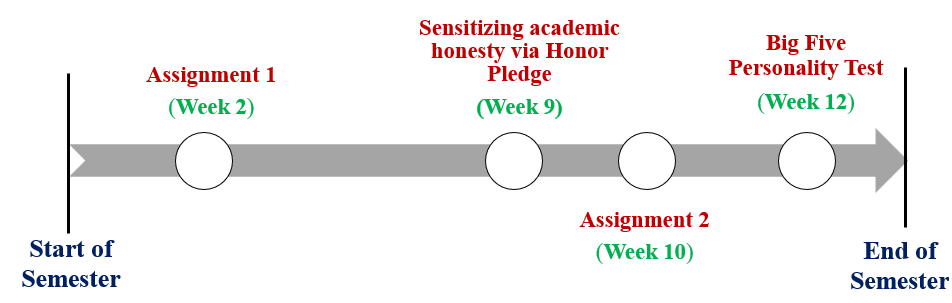
\includegraphics[width=\columnwidth]{SeriesOfactivities.png}}\vspace{-8pt}
  \caption{Series of activities}
  \label{fig:activityTimeline} \vspace{-10pt}
\end{figure}

 The data on personality traits and plagiarism scores, obtained through the Measure of Software Similarity (MOSS) for assignment 1, were utilized to address research question RQ\ref{RQ1}.

In the ninth week, all students had to read and endorse an honor/integrity pledge concerning plagiarism and collusion. This was aimed at raising awareness about plagiarism and upholding academic integrity. It explicitly outlined the behaviors considered plagiarism and collusion. The pledge was administered via a Google form, and a digital signature was mandated from each participant, signifying their commitment to refraining from plagiarism and collusion. Instead of in-class instruction, we opted for this method to ensure that all participants had sufficient time to comprehend the concepts of plagiarism and collusion without sacrificing any class time. The pledge remained accessible for a week and was mandatory. An excerpt from the honor pledge is provided below:

\begin{myquote}
    \textit{The assignments are to be done individually by each student. The objective of the assignments is to help students deepen their understanding of some of the concepts in AI. A secondary objective of the assignments is to help students get better at Python programming.}
    \textbf{Each} of the following amounts to violations of academic integrity:
    \begin{itemize}
        \item \textit{Sharing a part or whole of your program with another student even if one of the students changes the variable names and function names and rearranges the functions within the program file.}
        \item \textit{Sharing a part or whole of your report with another student even if one of the students changes most of the sentences so that superficially, the reports look different. You must cite the resources you have referred in the report.} 
        \item \textit{Getting parts of your program from past programming assignment submissions or internet sources. Each student must do the assignment individually.}
        \item \textit{Sharing code for commonly needed functionality by calling it "driver program" amounts to a violation of academic integrity because one of the objectives of this assignment is to help students get better at Python programming. }
    \end{itemize}
\end{myquote}
The second assignment served as the post-intervention assessment, allowing for the evaluation of the impact of plagiarism awareness on participant behavior.

Both programming assignments were original and did not have pre-existing solutions available on the internet. Below, we provide a brief overview of each assignment for the reader's understanding:

\subsubsection{First Programming Assignment:} The assignment centered on multi-armed bandit concepts and the Markov reward process. Students were tasked to develop a driver program that applied the concepts learned in class. Specifically, they were required to create a Python program capable of adjusting parameters within a provided AI model and visually representing the alterations on a graph. Additionally, students had to report all the findings along with the conclusion and rationale (as comments in the code). All relevant parameters and anticipated outcomes were covered in class, with the professor and teaching assistants available for any inquiries, during the designated assignment period via office hours. The following are the assignment's learning outcomes (LO) with their corresponding Revised Bloom Taxonomy \cite{bloomsTaxonomy} verbs in bold:
\begin{itemize}
    \item \textbf{Understand and Apply} multi-armed bandit and Markov reward process concepts. 
    \item \textbf{Analyze} parameter manipulation and visualization techniques. 
    \item \textbf{Implement} python programs efficiently 
\end{itemize}

\subsubsection{Second Programming Assignment:} The second assignment was based on the game `Connect 4'\footnote{\url{https://en.wikipedia.org/wiki/Connect_Four}}. Specifically, students were given the stub code for one version of the game that they could play and were tasked with modifying and enhancing the given program incrementally that plays against a Myopic player (a player that only views a fixed number of possibilities to evaluate a game state and not all possibilities) using the game tree-based search techniques and constraints given. Also, the students were given clear guidelines and steps to incrementally improve their player function by techniques like `Alpha-Beta Pruning'. The following are the assignment's LO's:
\begin{itemize}
    \item \textbf{Apply} game tree-based techniques and alpha-beta pruning effectively.
    \item \textbf{Implement} an incremental solution with retrospection after each stage.  
    \item \textbf{Comprehend} given python program and enhance it.
\end{itemize}

\subsection{Procedures for data collection and analysis}
\subsubsection{Personality Traits Data:} Following the institute's Human Ethical Committee (HEC) policy, participants were required to provide informed consent before participating in the study. Upon obtaining consent, participants underwent the International Personality Item Pool (IPIP) personality test, which assesses the Big Five personality traits. The test was administered through an online tool available at the provided URL\footnote{\url{https://bigfive-test.com/}}.

After completing the test, participants' final scores for each Big Five personality trait were recorded in a Google form after obtaining the informed consent form as approved by the HEC. To ensure confidentiality and protect participants' privacy, all data collected was anonymized, meaning any personally identifiable information was removed or obscured.

\subsubsection{Assignment Data:} 
Both assignments were administered using Moodle, the institute's learning management system. Upon completion, the source codes for both assignments were subjected to analysis using the Measure of Software Similarity (MOSS) tool to generate plagiarism reports.

To ensure confidentiality, the data was anonymized before processing. The plagiarism scores corresponding to each student (either via collusion or direct plagiarism from other sources), derived from the MOSS reports, were then stored in cloud storage for subsequent analysis. The plagiarism score for each student was calculated based on the proportion of code similarity detected by MOSS. Specifically, it was determined by dividing the maximum number of lines copied from other sources by the total number of lines in the student's source code (ignoring the empty lines). This approach provided a quantitative measure of the extent of plagiarism in each student's assignment.

% !TeX root = main.tex
\section{Results}
\label{sec:findings}
This section presents the study's descriptive and inferential statistics results, followed by a discussion of the findings.

The results of descriptive statistics revealed that 9\% of the participants rated extraversion, 14\% rated neuroticism, 17\% rated openness to experience, 28\% rated agreeableness, and 32\% rated conscientiousness as their dominant personality traits. Most participants exhibited high scores across various personality traits: 99\% scored high in Openness, indicating a proclivity for curiosity and imagination. Similarly, 91.32\% scored high in Extraversion, suggesting a preference for social interaction and enthusiasm. However, a substantial portion, 81.9\%, scored high in Neuroticism, indicating a tendency towards negative emotions and stress. Additionally, 88.57\% scored high in Agreeableness, reflecting a propensity for kindness and cooperation, while 81.1\% scored high in Conscientiousness, implying traits such as organization and responsibility. Table \ref{tab:correl} shows the pearson's correlations between the big-five personality traits. 

\vspace{-4pt}
\begin{table}[h]
  \centering
  \caption{Correlations between the Big-Five Traits\label{tab:correl}}
  \vspace{-12pt}
  \begin{tabular}{p{3cm}rrrrr}
    \toprule
    Trait & N & E & O & A & C \\\midrule
    Neuroticism (N) & 1.00 & -0.35 & 0.00 & -0.09 & -0.48 \\
    Extraversion (E) & -0.35 & 1.00 & 0.17 & 0.05 &	0.22 \\
    Openness (O) & 0.00 & 0.17 & 1.00 &	0.15 & -0.07 \\
    Agreeableness (A) & -0.09 &	0.05 & 0.15 & 1.00 & 0.43 \\ 
    Conscientiousness (C) & -0.48 & 0.22 & -0.07 &	0.43 &	1.00  \\\bottomrule
  \end{tabular}\vspace{-8pt}
\end{table}

Additionally, utilizing the plagiarism scores obtained from MOSS for both assignments, students were categorized into plagiarism levels according to the criteria outlined by the University Grants Commission (UGC) \cite{UGCPlagiarism}, a statutory body overseeing higher education in India. The outcomes are detailed in table \ref{tab:levelsPlagiarism}.


\begin{table}[h]
  \centering
  \caption{Percentage of students (out of N=105) falling in each Levels of Plagiarism \label{tab:levelsPlagiarism}}
  \vspace{-12pt}
  \begin{tabular}{p{1cm}p{2cm}rr}
    \toprule
    Level & Similarity \% & Assignment 1 & Assignment 2 \\\midrule
    Level 0 & Less than 10\% & 44.76\% & 40.95\% \\
    Level 1 & 10\% to 40\% & 27.51\% & 40.00\%  \\
    Level 2 & 41\% to 60\% & 14.28\% & 7.61\% \\
    Level 3 & More than 60\% &13.33\% & 11.42\% \\ \bottomrule
  \end{tabular}\vspace{-8pt}
\end{table}

\subsection{Influence of Big-Five traits on Plagiarism}

One of the linear multiple regression assumptions is that the independent variables must not exhibit high (>5) multicollinearity. The multicollinearity between the five personality traits was tested using the variance inflation factor (VIF) and shown in Table \ref{tab:VIF}. All the VIF values were less than 5, indicating that multiple linear regression can be performed. 

\begin{table}[h]
  \centering
  \caption{Big-Five traits and their VIF\label{tab:VIF}}
    \vspace{-12pt}
  \begin{tabular}{p{2cm}r}
    \toprule
    Trait & VIF Value \\\midrule
    Neuroticism & 1.46 \\
    Extraversion & 1.20 \\
    Openness & 1.10\\
    Agreeableness & 1.33 \\ 
    Conscientiousness & 1.70  \\\bottomrule
  \end{tabular}\vspace{-4pt}
\end{table}

Multiple linear regression analyses were conducted, with the big-five personality traits serving as the independent variables and the plagiarism score as the dependent variable for both assignments. The ordinary least squares (OLS) method, a statistical technique used to estimate the relationship between independent and dependent variables, was utilized for the analysis. The dependent variable was plagiarism score and the independent variables were the personality traits. The outcomes are displayed in Tables \ref{tab:assign1Regression} and \ref{tab:assign2Regression}. 

\begin{table}[h]
  \centering
  \caption{Regression analysis on Assignment 1 with $R^2$=0.106\\\label{tab:assign1Regression}}
    \vspace{-16pt}
  \begin{tabular}{p{2.5cm}llll}
    \toprule
    Trait & $\beta$ Coef & Std Err & \textit{t} & \textit{p}\\\midrule
    Agreeableness & 0.3489 & 0.243 & 1.434 & 0.155 \\
    Openness & -0.3401 & 0.256 & -1.328 & 0.187 \\
    Neuroticism & -0.1314 & 0.197 & -0.666 & 0.507 \\
    Extraversion & 0.6078 & 0.216 & 2.809 & 0.006** \\
    Conscientiousness & -0.2667 & 0.239 & -1.114 & 0.026* \\\bottomrule
  \end{tabular}\vspace{-4pt}
\end{table}

$\beta$ Coef represents the change in the dependent variable per one-unit change in the independent variable. Std Err gauges the variability of the $\beta$ coefficient. \textit{`t'} denotes the ratio of the $\beta$ coefficient to its standard error. p-value indicates significance, with `*' for \emph{p} < 0.05 and `**' for \emph{p} < 0.01.

\begin{table}[h]
  \centering
  \caption{Regression analysis on Assignment 2 with $R^2$=0.128\\\label{tab:assign2Regression}}
    \vspace{-16pt}
  \begin{tabular}{p{2.5cm}llll}
    \toprule
    Trait & $\beta$ Coef & Std Err & \textit{t} & \textit{p}\\\midrule
    Agreeableness & 0.3291 & 0.211 & 1.561 & 0.122 \\
    Openness & -0.3750 & 0.222 & -1.691 & 0.094\\
    Neuroticism & -0.2919 & 0.171 & -1.708 &  0.091\\
    Extraversion & 0.4394 & 0.187 & 2.344 & 0.021*\\
    Conscientiousness & -0.5541 & 0.207 & -2.673 & 0.009**\\\bottomrule
  \end{tabular}\vspace{-4pt}
\end{table}

Based on the findings from both assignments, irrespective of the actual coefficient values, it is apparent that extraversion exhibits a positive association with plagiarism (\textit{p}<0.05), while conscientiousness demonstrates a negative association with plagiarism (\textit{p}<0.05). However, the effect of the remaining personality traits are not statistically significant (\textit{p} values greater than 0.05).

\vspace{8pt}
\begin{mdframed}
\textbf{\textit{RQ1 Answer:}} Extraversion and conscientiousness traits influence plagiarism, with extraversion positively associated and conscientiousness negatively associated. The other three traits do not show a significant influence on plagiarism. 
\end{mdframed}
\vspace{8pt}

Some of these observations align with those reported in the literature, as illustrated in Table \ref{tab:litSUmmary}. For example, the lack of significance for openness to experience and neuroticism, as well as the negative association of conscientiousness with plagiarism, are consistent with the findings of Wilks et al. \cite{Wilks2016-WILPTA-3} and Giluk et al. \cite{Giluk2015BigFP}. 

However, in our study, extraversion demonstrates a positive association with plagiarism, consistent with the findings of Bhutto et al. \cite{Bhutto2019ACS} as shown in Fig \ref{fig:personalityAndPlagiarism}. 

\begin{figure}[H]
  \centering
  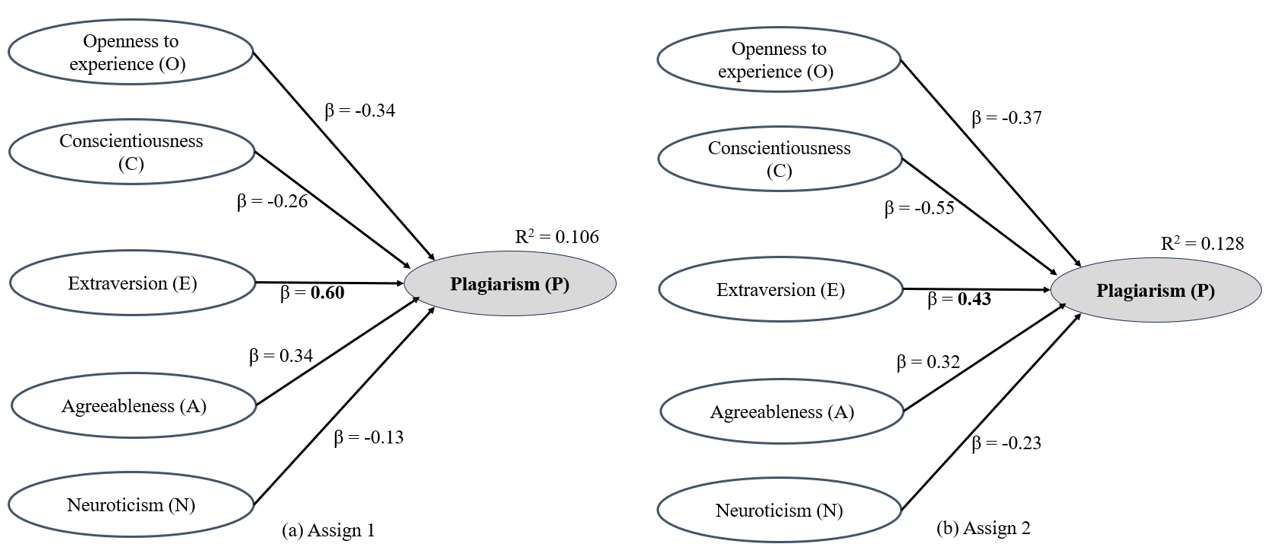
\includegraphics[width=\columnwidth]{1.png}
  \caption{The relationship between the big five traits and plagiarism in (a) Assign 1 and (b) Assign 2}
  \Description{In both of them, extroversion has a positive influence and openness to experience, and conscientiousness and neuroticism negatively influence plagiarism scores.}
  \label{fig:personalityAndPlagiarism}\vspace{-4pt}
\end{figure}

\subsection{Student behavior after sensitization via Honor Pledge }

The normality of plagiarism scores for Assignment 1 and Assignment 2 was assessed using histograms and the Shapiro-Wilk test, confirming their normal distribution. Our null hypothesis suggested that there would be no change in the mean percentage of similar lines of code after students were sensitized through an honor pledge for the second programming assignment. Given that we were comparing scores from the same students pre-intervention (Assignment 1 plagiarism scores) (N=105, Mean=23.45; SD=26.25) and post-intervention (Assignment 2 plagiarism scores) (N=105, Mean=21.23; SD=23.02), we conducted a paired t-test, \textit{t}(105) = 0.89, \emph{p} = 0.374, d = 0.0899. As p>0.05, we did not reject the null hypothesis. Here, the intervention refers to the honor pledge discussed earlier (See Sec 4).

As depicted in Table \ref{tab:levelsPlagiarism}, there was a slight decrease in the percentage of students falling in levels 2 and 3 of plagiarism after the intervention. While there was a marginal decline in the average plagiarism percentage from Assignment 1 to Assignment 2 (from 23.44\% to 21.22\%), the effect size computed using Cohen's d was weak (d=0.08). 

\vspace{4pt}
\begin{mdframed}
\textbf{\textit{RQ2 Answer:}} Our findings suggest that while educating students about plagiarism and collusion via an honor pledge may have some effect, its effectiveness in reducing plagiarism and collusion in programming assignments is limited as long as opportunities and pressure to engage in such behavior persist.
\end{mdframed}
\vspace{4pt}

We then specifically conducted the test for students who were involved in plagiarism and/or collusion in Assignment 1, those with a similarity score greater than 10\% (those falling into levels 1, 2, and 3 in Assignment 1, as shown in Table \ref{tab:levelsPlagiarism}). This allowed us to evaluate whether the intervention benefited students who engaged in such academic misconduct in Assignment 1, as they are the ones who might benefit most from such intervention. The paired sample t-test revealed a significant difference: the percentage of similarity score in Assignment 1 (N=58, Mean=41.73, SD=21.44) was notably higher than in Assignment 2 (N=58, Mean=28.92, SD=26.27); \textit{t}(57)=3.52, p=0.0008, D=0.53 (moderate effect). Similarly, when the t-test was performed only on those who did \emph{not} plagiarize and/or were involved in collusion, i.e., those whose similarity score was <10\% in assignment 1 (N=47, Mean = 0.21, SD=1.45) and assignment 2 (N=47, Mean=11.12, SD=12.56); \textit{t}(46)=5.8, p= 0.0000002, d=1.27.

While the findings regarding the significant impact of the intervention in reducing plagiarism and/or collusion on subsets of students (when considering those who were not involved separately) are compelling, it's essential to acknowledge the limitations and interpret the results with caution. Firstly, this result is not definitive as the intervention is not significant on the whole set of students (N=105) and should be further validated through replication studies, especially when considering these specific subcategories of students. Additionally, it's noteworthy that this outcome was not originally hypothesized, indicating the need for a deeper understanding of the underlying factors driving these effects.

\section{Discussion} \label{sec:discuss}

In this section, we examine our findings in light of the fraud triangle theory.

Our findings indicate that individuals with high extraversion scores demonstrate a greater tendency to engage in collusion to perform better in programming assignments. This propensity aligns with the fraud triangle model, where heightened extraversion fosters sociability and potentially larger social circles and friends, thereby increasing \emph{opportunities} for collusion. Moreover, extroverted individuals may find it easier to \emph{rationalize} their actions as commonplace due to their sociable nature.

Also, in both assignments, the students were not provided explicit information regarding the plagiarism checks that would be conducted using MOSS for their solutions. Students perceived that there was still an \emph{opportunity} for plagiarism. Our results indicate that sensitizing students about plagiarism did not lead to a significant reduction in such behavior. Students continue to plagiarize through collusion as long as they perceive an \textit{opportunity} and/or are \textit{pressured} to do so. Consequently, the impact of the honor pledge on reducing plagiarism was perceived as weak.

The correlation between the extraversion trait tending to plagiarise, making use of the opportunity, and plagiarism in India's academic environment can be understood within the \textit{pressure} aspect of the fraud triangle model. In this model, pressure refers to the internal or external forces that compel individuals to engage in misconduct. In Indian society, there is often a strong emphasis on competitiveness and achievement, particularly in academic settings where grades and academic success are highly valued \cite{IITPrepMenace,UnemploymentIndia, NAIR2020831}. %. For instance, prestigious institutions like the IITs, which are top-ranked according to the National Institutional Ranking Framework (NIRF), the official framework for ranking higher education institutes across India \footnote{\url{https://www.nirfindia.org/2023/EngineeringRanking.html}}, receive applications from over one million students every year for a limited number of seats, typically around 10,000. This intense competition and pressure to excel start early, with students enrolling in specialized coaching institutes for exam preparation as young as ten years old \cite{IITPrepMenace}. 

%Furthermore, the pressure to obtain employment is aggravated by the harsh realities of the job market. India has approximately 2 million computer science students, with ongoing concerns regarding employability rates, which can drop to as low as below 25\% \cite{UnemploymentIndia, NAIR2020831}. As a result, many students encounter challenges in securing suitable job opportunities. 
The pressure to succeed in this fiercely competitive environment and pressure stemming from societal expectations, family aspirations, and the intense competition for limited opportunities may drive individuals to resort to unethical practices like plagiarism and collusion to gain a competitive edge. The significant number (81.9\%) displaying a high neuroticism score implies a likelihood of participants experiencing stress and anxiety, highlighting the role of pressure. This environment fosters a mentality of optimizing results by any means necessary. Thus, the propensity for plagiarism is driven more by opportunity than rationale, as students feel pressured to perform. 

Our results suggest that individuals exhibiting higher levels of conscientiousness tend to show reduced inclinations toward plagiarism. This observation is consistent with the fraud triangle model. Conscientious individuals prioritize diligence and self-discipline, making them less prone to exploiting opportunities for plagiarism and less likely to rationalize such behavior, even under pressure.

These factors collectively imply that plagiarism and collusion in assignments may result from a blend of cultural, societal, and educational influences shaping individuals' attitudes and behaviors regarding academic integrity. Moreover, an honor pledge appears to have limited efficacy in enhancing academic integrity.
\vspace{-4pt}

% !TeX root = main.tex
\section{Limitations and Future Work}
\label{sec:limitations}
This study has several limitations that should be noted. As a result, the findings may not be directly applicable to other educational environments or programming tasks that differ significantly in scope and complexity.

\begin{itemize}
    \item \textit{Single Institution Context:} Our study was conducted in a single institution in India, which may limit the generalizability of our findings. Different educational settings and cultures may influence the effectiveness of the honor pledge intervention.
    \item \textit{Sample Size and Demographics:} The relatively small sample size of 105 students may not capture the diversity of student behavior and attitudes toward plagiarism. Larger, more diverse samples are needed to validate our findings.
    \item \textit{Influence of Pre-existing Academic Integrity Culture:} The existing academic integrity culture at the institution may have influenced the outcomes. Institutions with different levels of emphasis on academic integrity might experience different results from the intervention.
    \item \textit{Impact of External Factors:} As discussed in the discussion, external factors, such as peer influence, \textit{pressure} to excel, perceived \textit{opportunity}, and the difficulty of the assignments, could have contributed to the outcomes. These factors were not controlled for in the study and may have influenced the results.
    \item \textit{Comparison of Different Types of Assignments:} Our study focused on two programming assignments, which may not be representative of all types of assignments. The nature of the assignments and the presence of code stubs or templates could affect the incidence of plagiarism and the effectiveness of the honor pledge. We tried to reduce the severity of this issue by using the -b parameter while executing MOSS as discussed in Sec \ref{sec:method}.
    \item \textit{Absence of Control Group:} We could have designed the experiment with two groups – a control group and an honor pledge group – for each of the two programming assignments. However, we felt that the results would be difficult to interpret if collusion occurred between students of different groups. For example, if a student from the control group colluded with a student from the honor pledge group, it would complicate the interpretation of the results. Therefore, we avoided using separate groups and the current study focuses only on comparing the percentage of code similarity across two different programming assignments. Although we avoided using separate control and honor pledge groups to prevent collusion and interpretational difficulties, this decision introduces a potential confounding variable. Future studies with a clear control group could provide more robust evidence of the honor pledge's effectiveness.
    \item \textit{Random Chance and Personality Traits:} The cross-sectional design of the study limits our ability to establish causal relationships between personality traits and plagiarism behavior. It is possible that, due to random chance, participants who engaged in plagiarism in both programming assignments had higher scores for the extraversion personality trait. This could result in a positive correlation between extraversion and the percentage of code similarity across both programming assignments.
    \item \textit{Gender Distribution and Cultural Homogeneity:} In India, engineering programs exhinit a severe imbalance in gender represention. For example, at our institution, only 12.5\% of the undergraduate students in the computer science program identify as female. The same is reflected in this study with only 6.6\% of participants being female. This disproportionate gender distribution (98 men to 7 women) and cultural homogeneity (all participants from India) may limit the generalizability of the study's findings to other demographic groups or cultural contexts.  
    \item \textit{Personality Test Timing:} Administering the personality test after the second assignment (at the end of the semester) might not accurately reflect the personality traits, as experiences from the course or external factors could alter trait expressions \emph{temporarily}.
\end{itemize}

Furthermore, the study primarily relied on quantitative analysis, overlooking the nuanced qualitative aspects of students' perceptions and experiences regarding plagiarism and collusion which could bring about contextual factors, such as cultural norms and academic pressures, which may influence plagiarism behavior.

Future research endeavors could address these limitations by incorporating qualitative interviews to gain deeper insights into students' attitudes, motivations, and plagiarism-related experiences. Longitudinal studies could provide a more comprehensive understanding of the dynamics between personality traits and plagiarism behavior over time, particularly following interventions aimed at sensitizing students about plagiarism. Additionally, replicating the study in diverse educational settings and cultural contexts could enhance the robustness of the findings and improve generalizability.
 

% !TeX root = main.tex
\section{Conclusion}
\label{sec:conclusion}

In conclusion, our study involving 105 students in India revealed significant insights into the influence of personality traits on plagiarism and the effectiveness of sensitizing students about plagiarism via an honor pledge in mitigating academic misconduct. Our findings underscored that extraversion and conscientiousness traits play pivotal roles in shaping plagiarism behavior, with extraversion positively associated and conscientiousness negatively associated with plagiarism. However, the impact of educational interventions on reducing plagiarism was found to be limited. This aligns with the framework of the fraud triangle, which emphasizes the role of rationalization, opportunity, and pressure in fostering fraudulent behavior. In the highly competitive academic landscape of India, where pressure to excel is pronounced, addressing underlying pressures faced by students emerges as a critical strategy for promoting academic integrity. Therefore, our study highlights the importance of adopting comprehensive approaches that not only focus on sensitizing students about plagiarism but also address the underlying pressures contributing to academic misconduct.

\bibliographystyle{ACM-Reference-Format}
\bibliography{main.bib}

% \section{Appendices}

% Uncomment if required.

\end{document}
\endinput
%%
%% End of file `sample-authordraft.tex'.
